\newcommand{\nom}{Porte conteneur}
\newcommand{\sequence}{03}
\newcommand{\num}{04}
\newcommand{\type}{TD}
\newcommand{\descrip}{Résolution d'un problème en utilisant des méthodes algorithmiques}
\newcommand{\competences}{Alt-C3: Concevoir un algorithme répondant à un problème précisément posé}
\documentclass[10pt,a4paper]{article}
  \usepackage[french]{babel}
  \usepackage[utf8]{inputenc}
  \usepackage[T1]{fontenc}
  \usepackage{xcolor}
  \usepackage[]{graphicx}
  \usepackage{makeidx}
  \usepackage{textcomp}
  \usepackage{amsmath}
  \usepackage{amssymb}
  \usepackage{stmaryrd}
  \usepackage{fancyhdr}
  \usepackage{lettrine}
  \usepackage{calc}
  \usepackage{boxedminipage}
  \usepackage[french,onelanguage, boxruled,linesnumbered]{algorithm2e}
  \usepackage[colorlinks=false,pdftex]{hyperref}
  \usepackage{minted}
  \usepackage{url}
  \usepackage[locale=FR]{siunitx}
  \usepackage{multicol}
  \usepackage{tikz}
  \makeindex

  %\graphicspath{{../Images/}}

%  \renewcommand\listingscaption{Programme}

  %\renewcommand{\thechapter}{\Alph{chapter}}
  \renewcommand{\thesection}{\Roman{section}}
  %\newcommand{\inter}{\vspace{0.5cm}%
  %\noindent }
  %\newcommand{\unite}{\ \textrm}
  \newcommand{\ud}{\mathrm{d}}
  \newcommand{\vect}{\overrightarrow}
  %\newcommand{\ch}{\mathrm{ch}} % cosinus hyperbolique
  %\newcommand{\sh}{\mathrm{sh}} % sinus hyperbolique

  \textwidth 160mm
  \textheight 250mm
  \hoffset=-1.70cm
  \voffset=-1.5cm
  \parindent=0cm

  \pagestyle{fancy}
  \fancyhead[L]{\bfseries {\large PTSI -- Dorian}}
  \fancyhead[C]{\bfseries{{\type} \no \numero}}
  \fancyhead[R]{\bfseries{\large Informatique}}
  \fancyfoot[C]{\thepage}
  \fancyfoot[L]{\footnotesize R. Costadoat, C. Darreye}
  \fancyfoot[R]{\small \today}
  
  \definecolor{bg}{rgb}{0.9,0.9,0.9}
  
  
  % macro Juliette
  
\usepackage{comment}   
\usepackage{amsthm}  
\theoremstyle{definition}
\newtheorem{exercice}{Exercice}
\newtheorem*{rappel}{Rappel}
\newtheorem*{remark}{Remarque}
\newtheorem*{defn}{Définition}
\newtheorem*{ppe}{Propriété}
\newtheorem{solution}{Solution}

\newcounter{num_quest} \setcounter{num_quest}{0}
\newcounter{num_rep} \setcounter{num_rep}{0}
\newcounter{num_cor} \setcounter{num_cor}{0}

\newcommand{\question}[1]{\refstepcounter{num_quest}\par
~\ \\ \parbox[t][][t]{0.15\linewidth}{\textbf{Question \arabic{num_quest}}}\parbox[t][][t]{0.85\linewidth}{#1\label{q\the\value{num_quest}}}\par
~\ \\}

\newcommand{\reponse}[4][1]
{\noindent
\rule{\linewidth}{.5pt}\\
\textbf{Question\ifthenelse{#1>1}{s}{} \multido{}{#1}{%
\refstepcounter{num_rep}\ref{q\the\value{num_rep}} }:} ~\ \\
\ifdef{\public}{#3 ~\ \\ \feuilleDR{#2}}{#4}
}

\newcommand{\cor}
{\refstepcounter{num_cor}
\noindent
\rule{\linewidth}{.5pt}
\textbf{Question \arabic{num_cor}:} \\
}



\begin{document}

\begin{center}
{\Large\bf TP \no {\num} -- \descrip}
\end{center}

\SetKw{KwFrom}{de} 

\noindent L'objectif de ce TD est de r\' esoudre num\' eriquement des \' equations du type $f(x)=0$ avec $f\colon \mathbb{R}\to \mathbb{R}$ suppos\' ee continue. On utilisera pour \c ca deux algorithmes : la m\' ethode par dichotomie et la m\' ethode de Newton.

\section{Dichotomie}
Lors du TP n°7, vous avez \' ecrit une fonction \verb?dicho? qui prend comme entr\' ee la fonction \` a \' etudier, les bornes initiales $a$ et $b$, la pr\' ecision $\epsilon$ et qui renvoie $\dfrac{a_n+b_n}{2}$, approximation d’une solution \` a $\epsilon$ pr\` es. Retrouvez cette fonction et sauvegardez-la dans votre nouveau programme du TP n°\num.

\section{M\' ethode de Newton}
\subsection{Principe de la m\' ethode}
\noindent La m\' ethode de Newton est un algorithme qui permet d'obtenir une approximation d'une solution $\alpha$ de l'\' equation $f(x)=0$.\\
Partant d'un point $x_0$, on consid\` ere la tangente \` a la courbe en $x_0$ :
\[T_{x_0}\colon y = f(x_0)+f'(x_0)(x-x_0)\]
Elle intersecte l'axe des abscisses en $x_1$ : $0=f(x_0)+f'(x_0)(x_1-x_0) \Leftrightarrow x_1=x_0-\dfrac{f(x_0)}{f'(x_0)}$.\\
Sous certaines conditions, $x_1$ peut \^ etre une meilleure approximation de $\alpha$ que $x_0$.
\begin{center}
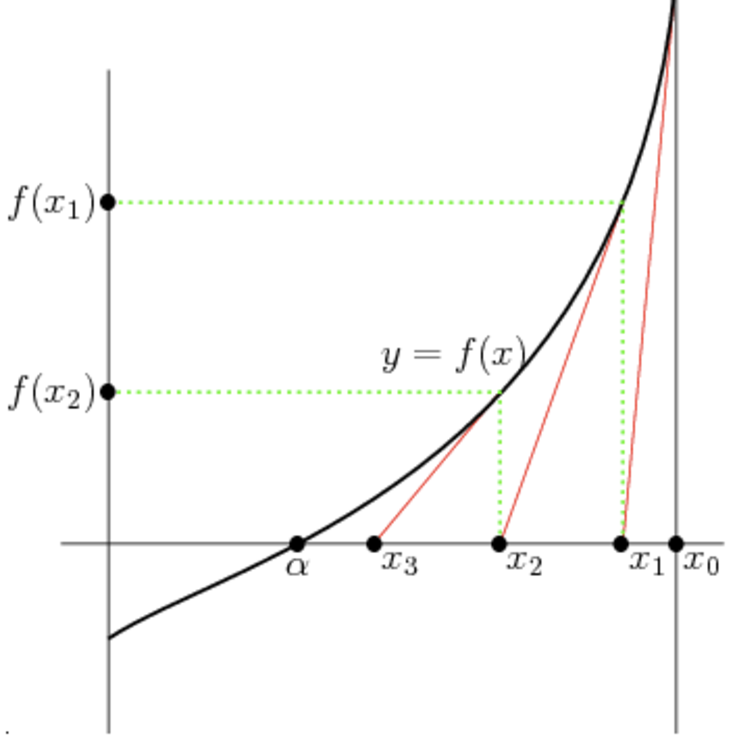
\includegraphics[scale=0.5]{Dessin/Newton_convexe.pdf}
\end{center}
On construit ainsi de mani\` ere r\' ecurrente la suite $(x_n)_{n\in\mathbb{N}}$ d'approximations de $\alpha$ : 
\[x_{n+1}=x_n-\dfrac{f(x_n)}{f'(x_n)}\]
\textbf{Avantage }: quitte \` a ne pas \^ etre trop \' eloign\' e de la solution et avec des hypoth\` eses raisonnables sur $f$, la convergence est tr\` es rapide. On dit qu'elle est quadratique.\\
\textbf{Inconv\' enients }:
\begin{enumerate}
\item la m\' ethode ne converge pas n\' ecessairement. Notamment, si $f'$ s'annule ou devient tr\` es petit, on peut avoir des probl\` emes avec la division par $f'(x_n)$.\\
Elle peut aussi "boucler" de mani\` ere infinie. 
\item On a plusieurs choix pour le test d'arr\^ et de l'algorithme :
\begin{enumerate}
\item on se fixe un nombre d'it\' erations de la boucle ;
 \item \` a $\epsilon>0$ fix\' e, le crit\` ere d'arr\^ et est : $|x_{n+1}-x_n|\leqslant \epsilon$. \\
 Le test peut \^ etre valid\' e sans pour autant que $x_n$ soit une approximation de $\alpha$ \` a $\epsilon$ pr\` es, mais en g\' en\' eral, cela fonctionne bien.
 \item $|f(x_n)|\leqslant \epsilon$. L\` a encore, $f$ peut \^ etre petite en $x_n$ mais ne pas s'annuler pr\` es de $x_n$.
 \end{enumerate}
\noindent Comme il y a un risque que la m\' ethode de Newton ne converge pas, on mettra toujours dans le test d'arr\^ et un nombre d'it\' erations maximal.
\item Il faut connaitre $f'$.
\end{enumerate}


\subsection{Applications}
\begin{exercice}
\begin{enumerate}
\item Ecrire une fonction \verb?Newton1? qui prend comme entr\' ee la fonction \` a \' etudier, sa d\' eriv\' ee, une valeur initiale de la suite $x_0$ et un nombre d'it\' erations $n$ et qui renvoie $x_n$ approximation d'une  solution.
\item Testez cette fonction sur $f\colon x\mapsto x^2-2$ avec diff\' erentes valeurs de $x_0$ et de $n$.
\item Que se passe-t-il si vous prenez $x_0=0$ ? Pourquoi ?
\item La suite $(x_n)$ peut converger vers $\sqrt{2}$ ou $-\sqrt{2}$. Au bout de combien d'it\' erations a-t-on une valeur approch\' ee de $\sqrt{2}$ \` a $10^{-10}$ pr\` es en partant de $x_0=2$ ? 
\end{enumerate}
\end{exercice}




\begin{exercice}
\label{exo newton diverge}
Appliquer \verb?Newton1? \` a la fonction $x\mapsto x^3-2x+2$ en d\' emarrant \` a $x_0=0$. Que se passe-t-il ? Quand vous avez une r\' eponse, reportez-vous au graphique en fin d'\' enonc\' e pour visualiser la suite $(x_n)$.\\
Que se passe-t-il si on d\' emarre avec un $x_0$ assez proche de $0$ ou $1$ ?
\end{exercice}



\begin{exercice}
Modifier la fonction \verb?Newton1? en une fonction \verb?Newton2? pour que le criti\` ere d'arr\^ et soit $|x_{n+1}-x_n|\leqslant \epsilon$. \\
La fonction \verb?Newton2? prendra comme entrée : la fonction \` a \' etudier $f$, sa d\' eriv\' ee $f'$, une valeur initiale de la suite $x_0$ et la marge d'erreur $\epsilon$. Pour éviter les boucles infinies, on fera en sorte que dans cette fonction, le nombre d'itérations ne dépasse pas $1 000$.
\end{exercice}



\begin{exercice}
Testez la fonction \verb?Newton2? sur $x\mapsto \sin(x)$ pour d\' eterminer une approximation de $\pi$. Comparer la valeur de $x_n-\pi$ avec la valeur $\epsilon$ choisie. Qu'en pensez-vous ?
\end{exercice}



\begin{exercice}Comparaison de la vitesse des deux m\' ethodes.\\
On veut comparer la vitesse des deux algorithmes, dichotomie et m\' ethode de Newton sur la fonction $f(x)=x^2-2$, avec une pr\' ecision $\epsilon=10^{-10}$.\\
Modifier les fonctions \verb?dicho? et \verb?Newton2? pour savoir laquelle est la plus rapide. Pour cela, on pourra comparer le nombre d'it\' erations effectu\' ees dans chaque programme ou le temps mis par chaque algorithme en utilisant la m\' ethode \verb?time()? de la biblioth\` eque \verb?time?.
\end{exercice}


\begin{exercice}Méthode dans le cas où on ne connait pas $f'$.\\
Il se peut qu'on ne connaisse pas la d\' eriv\' ee de $f$. Dans ce cas, on peut approximer $f'(x_n)$ par $\dfrac{f(x_n+h)-f(x_n)}{h}$ pour un $h$ fix\' e petit.\\
Modifier la fonction \verb?Newton2? en une fonction \verb?Newton3? qui a comme entr\' ee la fonction $f$, $x_0$, $\epsilon$, $h$ et qui renvoie $x_n$.
\end{exercice}




\begin{exercice}M\' ethode de la s\' ecante\\
Avec cette m\' ethode, on ne connait pas $f'$. On approxime $f'(x_n)$ par le coefficient directeur de la corde passant par $(x_n,f(x_n))$ et $(x_{n-1},f(x_{n-1}))$ : $f'(x_n)\approx \dfrac{f(x_{n})-f(x_{n-1})}{x_{n}-x_{n-1}}$\\
La relation de r\' ecurrence de la suite $(x_n)$ est donn\' ee par :
\[x_{n+1}=x_n-f(x_n)\dfrac{x_{n}-x_{n-1}}{f(x_{n})-f(x_{n-1})}\]
On a besoin de deux points $x_0$ et $x_1$ pour initialiser la suite $(x_n)$.\\
Ecrire une fonction \verb?secante? qui prend comme entrée $f$, $x_0,x_1$ et $\epsilon$ renvoie $x_n$.
\end{exercice}





\begin{exercice}M\' ethode de Newton en complexe.
\begin{enumerate}
\item Quelle sont les racines de la fonction $f(x)=x^2+1$ ? Testez la fonction \verb?Newton1? avec $f$ pour $x_0$ r\' eel puis un $x_0$ complexe. 
\item Les solutions complexes de l'\' equation $z^3=1$ sont :  $1\ ;\  -\dfrac{1}{2}+i\dfrac{\sqrt{3}}{2}\ ; \ -\dfrac{1}{2}-i\dfrac{\sqrt{3}}{2}$. A l'aide de la fonction \verb?Newton1?, retrouvez ces valeurs en choisissant un bon $x_0$.%GNA
\end{enumerate}
\end{exercice}



\newpage

\section{Annexe}
\subsection{Vitesse de convergence}
\noindent \textbf{Dichotomie :} chaque \' etape de l'algorithme, on divise la longueur de l'intervalle par 2. Si on note $\alpha$ le z\' ero de $f$, on a :
\[|c_{n+1}-\alpha|\leqslant \dfrac{1}{2}|c_n-\alpha|\]
On dit que la convergence est lin\' eaire.\bigskip \\
\textbf{M\' ethode de Newton :} avec des hypoth\` eses raisonnables sur $f$ (par exemple, $f'(\alpha)>0$ et $f''\geqslant 0$), alors il existe une constante $C$ telle que \` a partir d'un certain rang, 
\[|x_{n+1}-\alpha|\leqslant C|x_n-\alpha|^{2}\]
On dit que la vitesse de convergence est quadratique.\bigskip \\
\textbf{Exemple de comparaison des deux algorithmes :} Si on intialise les deux algorithmes en $x_0$ \` a une distance $\frac{1}{2}$ de $\alpha$ : \\
\[|c_n-\alpha|\leqslant \left(\dfrac{1}{2}\right)^{n+1}\]
\[|x_n-\alpha|\leqslant \left(\dfrac{1}{2}\right)^{2^n}\]
La m\' ethode de Newton est beaucoup plus rapide que la dichotomie.

\subsection{Illustration de l'exercice  \ref{exo newton diverge}}
\begin{center}
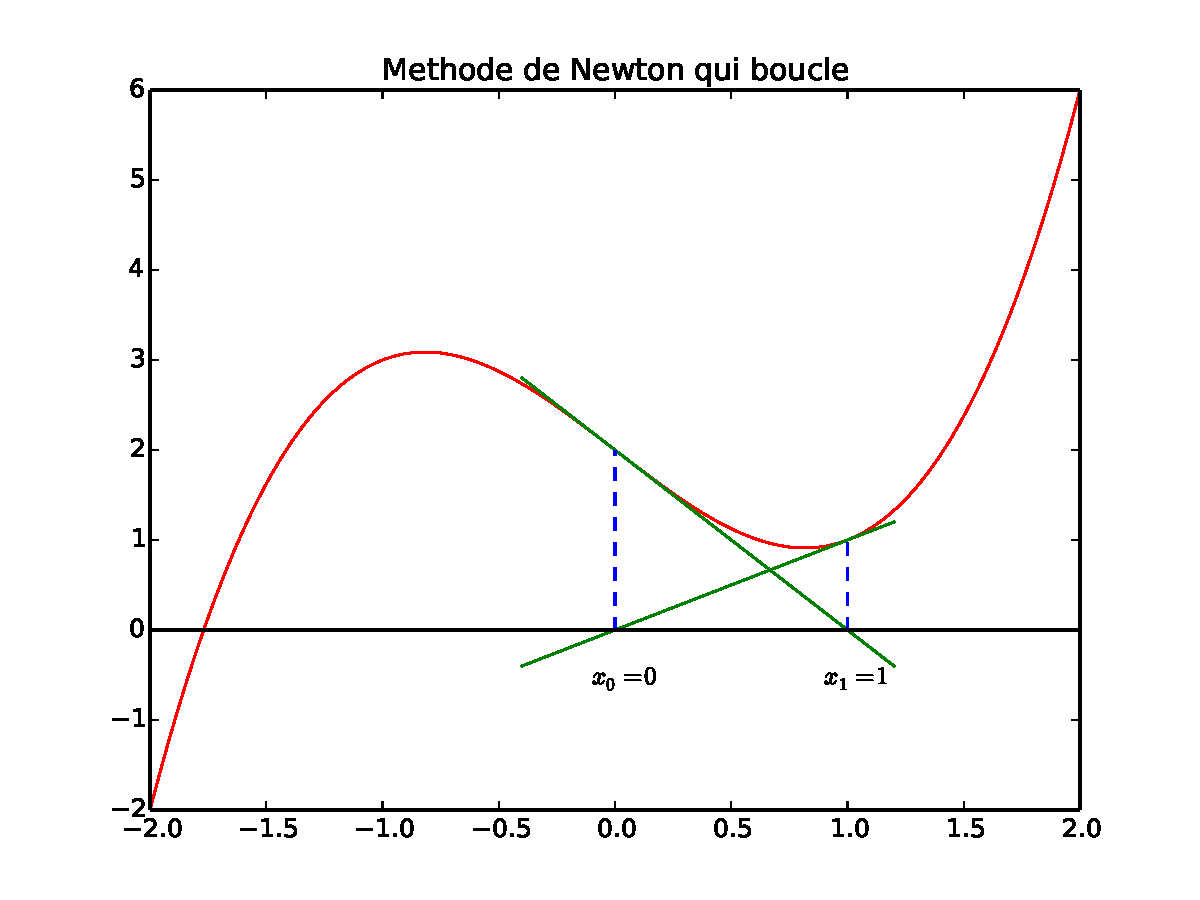
\includegraphics[scale=0.5]{Dessin/Newton_boucle.pdf}\\
La suite $(x_n)$ de l'exercice \ref{exo newton diverge}
\end{center}





\ifdef{\public}{\end{document}}{}

\newpage 

\begin{center}
{\Large\bf Correction TP \no {\num} -- \descrip}
\end{center}


\begin{solution}~\\
\vspace*{-0.7cm}
\begin{enumerate}
\item \begin{minted}[frame=lines]{python}
def Newton1(f,fprime,x0,nb_iteration):
    x=float(x0)
    for i in range(nb_iteration):
        x=x-f(x)/fprime(x)
    return(x) 
\end{minted}
\item \begin{minted}[frame=lines]{python}
def f(x):
    return(x**2-2)
def fprime(x):
    return(2*x)
\end{minted}
\item $f'(0)=0$ : Python renvoie un message d'erreur car il ne peut pas diviser par $0=f'(0)$.
\item Newton1$(f,f',2,3)-\sqrt{2}=O( 10^{-6})$ et Newton1$(f,f',2,4)-\sqrt{2}=O( 10^{-12})$.\\
Donc pour $n=4$, on a une approximation \` a $10^{-10}$ pr\` es.
\end{enumerate}
\end{solution}

\begin{solution}
La suite "boucle", elle vaut : $0,1,0,1,0,1,\cdots$\\
Les points $x=0$ et $x=1$ sont "supers attractifs" : si on initialise la suite assez pr\` es de ces valeurs, les termes de la suite vont converger vers 0 et 1. Pour Python, la suite va finir par boucler $0,1,0,\cdots$
\end{solution}


\begin{solution}~\\
\vspace*{-0.7cm}
\begin{minted}[frame=lines]{python}
def Newton2(f,fprime,x0,epsilon):
    x0=float(x0)
    x1=x0-f(x0)/fprime(x0)
    compteur=0    # on compte le nb d iterations de la boucle
    # test d arret : on itere la boucle si l ecart entre xn et x(n+1) est grand 
    # et si on a fait moins de 1000 iterations
    while abs(x1-x0)>epsilon and compteur<1000 : 
        x0=x1
        x1=x1-f(x1)/fprime(x1)
        compteur=compteur+1
    return(x1)  
\end{minted}    
Méthode 2 :    
\begin{minted}[frame=lines]{python}
def Newton2Bis(f,fprime,x0,epsilon):
    x=float(x0)
    compteur=0
    # l ecart entre xn et x(n+1) est f(xn)/fprime(xn)
    while abs(f(x)/fprime(x))>epsilon and compteur<1000 : 
        x=x-f(x)/fprime(x)
        compteur=compteur+1
    return(u)        
\end{minted}
\end{solution}

\begin{solution}
On teste : \verb?Newton2(sin,cos,2,1e-3)-pi?. On trouve $9.10^{-11}$.\\
La diff\' erence est bien inf\' erieure \` a $\epsilon$, elle est m\^ eme tr\` es inf\' erieure, car l'algorithme est tr\` es rapide.  
\end{solution}



\begin{solution}
On compare le nombre d'it\' erations et le temps mis par les deux algorithmes.
\begin{minted}[frame=lines]{python}
import time

def dicho_comparaison(f,a,b,eps):
    t=time.time()            # donne le temps de calcul
    compteur=0           # va compter le nombre d'iterations                
    if f(a)*f(b)>0:
        return('nous ne savons pas si f s annule entre a et b')
    while (b-a)>2*eps:
        compteur=compteur+1
        c=(float(a)+b)/2
        if f(a)*f(c)<0:
            b=c
        else:
            a=c     
    return((a+b)/2,time.time()-t,compteur)

def Newton_comparaison(f,fprime,u0,epsilon):
    t=time.time()             # donne le temps de calcul
    compteur=0           # va compter le nombre d'iterations        
    u0=float(u0)
    u1=u0-f(u0)/fprime(u0)
    while abs(u1-u0)>epsilon and compteur<1000 : 
        u0=u1
        u1=u1-f(u1)/fprime(u1)
        compteur=compteur+1
    return(u1,time.time()-t,compteur)      
\end{minted}
On teste ensuite sur la même fonction, avec la même marge d'erreur :
\begin{minted}[frame=lines]{python}
Newton_comparaison(carre,carre_prime,2,1e-15)
dicho_comparaison(carre,0,2,1e-15)
\end{minted}
\end{solution}


\begin{solution}~\\
\vspace*{-0.7cm}
\begin{minted}[frame=lines]{python}
def Newton3(f,h,x0,epsilon):
    x0=float(x0)
    derivee=(f(x0+h)-f(x0))/h
    x1=x0-f(x0)/derivee
    compteur=0
    while abs(x1-x0)>epsilon and compteur<1000 :
        x0=x1
        derivee=(f(x1+h)-f(x1))/h
        x1=x1-f(x1)/derivee
        compteur=compteur+1
    return(x1) 
\end{minted}
\end{solution}

\begin{solution}
Attention, il se peut que lorsque $x_{n+1}$ et $x_n$ sont trop proches, Python renvoie un message d'erreur car $f(x_{n})-f(x_{n-1})\approx 0$.
\begin{minted}[frame=lines]{python}
def secante(f,x0,x1,eps):
    x0=float(x0)
    x1=float(x1)
    compteur=0
    while abs(x0-x1)>eps and compteur<1000:
        temp=x1
        x1=x1-f(x1)*(x1-x0)/(f(x1)-f(x0))
        x0=temp
        compteur=compteur+1
    return(x1) 
\end{minted}
\end{solution}

\begin{solution}
Avec un $x_0$ r\' eel, l'algorithme ne converge pas. Avec un $x_0$ complexe, l'algorithme renvoie \verb?1j?.
\end{solution}

\end{document}